\subsection{Energy Balance Inequality.}
\label{sec_ine}
The energy imbalance inequality reads:
\begin{equation}
\frac{\d}{\d t} \left\{\int_R \psi \right\}\leq W(R) + M(R) \label{energyin}
\end{equation}
where $R$ is an arbitrary control volume of the system, $\psi$ is the Helmholtz free energy, $W(R)$ is the rate at which the environment does work on $R$ and $M(R)$ is the inflow of mass due to transport. Considering a control volume $R$ in the reference configuration $\mathcal{B}_0$, the system exchanges mass due to the diffusion of each mobile species, so that $M(R)$ is given by:
\begin{equation}
M(R)= \sum\limits_{m=s,1,\ldots,N} - \int_{\partial R} \mu_m \,\mathbf{J}_m \cdot \mathbf{n} 
\end{equation}
where $\mathbf{n}$ is the unit normal vector to the surface $\partial R$ and $\mu_m$ is the chemical potential associated with each species. Widely used in the thermodynamics of mixture, the chemical potential is a measure of the rate of change in free energy associated with adding one more molecule to a unit volume.

The term $W(R)$, i.e. the rate of work done on the system, is instead decomposed in two contributions, the rate of electrical $W_{el}(R)$ and mechanical work $W_{mec}(R)$. Following \cite{DROZDOVph}, $W_{el}(R)$ is defined as:
\begin{equation}
W_{el}(R) = -\int_{\partial R} \Phi\, \dot{\mathbf{H}}\cdot \mathbf{n}
\end{equation}

Following the work of Gurtin \cite{GURTIN}, we account both for the presence of macro-stresses $\mathbb{S}$ and micro-stresses $\boldsymbol{\xi}$, which arise due to the system heterogeneity \cite{microstress}\footnote{Assuming only interface is between solid and solvent phase.}. As before we only consider the dominant contribution of the solvent while neglecting the solute, so that $W_{mec}(R)$ reads:
\begin{equation}	\centering
%	\begin{subfigure}{0.32\textwidth}
%		\centering
%		\Large
%	\def\svgwidth{0.95\linewidth}
%	\input{latex/images/modelA1.pdf_tex}
%	\caption{Rheological Model A}
%	\label{fig1A}
%	\end{subfigure}
W_{mec}(R) = \int_{\partial R} \left(\boldsymbol{\xi}_1\cdot \mathbf{n}\right)\dot{C}_s + \int_{\partial R} \mathbb{S}\mathbf{n} \cdot \dot{\mathbf{u}}+  \int_{\partial R}\left(\boldsymbol{\xi}_2\cdot \mathbf{n}\right)\dot{J}
\end{equation}
where $\mathbf{u}= \mathbf{x}-\mathbf{X}$ is the displacement vector, which is related to the deformation tensor by $\F=\mathbb{I}-\nabla_0 \mathbf{u}$. Substituting this result back into the formula~(\ref{energyin}) and applying the divergence theorem we obtain the following inequality:
\begin{equation}
\int_R \dot{\psi} - \mathbf{E}\cdot \dot{\mathbf{H}} \, + \, \sum\limits_{i=1}^{N} \left[e \Phi  z_i \dot{C}_i+ \nabla_0 \left(\mu_i \mathbf{J}_i \right)\right] + \nabla_0 (\mu_s \mathbf{J}_s- \boldsymbol{\xi}_1\dot{C}_s- \boldsymbol{\xi}_2\dot{J} -\mathbb{S}^T\mathbf{\dot{u}}) \leq 0 
\end{equation}

Since this must hold for any choice of the volume $R$, the inequality must hold also locally:
\begin{equation}
\dot{\psi} - \mathbf{E}\cdot \dot{\mathbf{H}} \, + \, \sum\limits_{i=1}^{N} \left[e \Phi  z_i \dot{C}_i+ \nabla_0 \left(\mu_i \mathbf{J}_i \right)\right] + \nabla_0 (\mu_s \mathbf{J}_s- \boldsymbol{\xi}_1\dot{C}_s- \boldsymbol{\xi}_2\dot{J} -\mathbb{S}^T\mathbf{\dot{u}}) \leq 0. 
\end{equation}
Further accounting for Equations~(\ref{consmass})-(\ref{consmom}), we obtain that:
\begin{equation}
\begin{aligned}
\dot{\psi} - \mathbf{E}\cdot \dot{\mathbf{H}} \, + \, \sum\limits_{i=1}^{N} \left[e \Phi  z_i - \mu_i\right] \dot{C}_i - (\mu_s + \nabla_0 \cdot \boldsymbol{\xi}_1)\,\dot{C}_s -\left(\mathbb{S} +J\nabla_0 \cdot \boldsymbol{\xi}_2\F^{-1}\right):\dot{\F}\\
-\boldsymbol{\xi}_2 \cdot \nabla_0 \, \dot{J}-\boldsymbol{\xi}_1 \cdot \nabla_0 \, \dot{C}_s + \sum\limits_{m} \nabla_0 \, \mu_m \cdot \mathbf{J}_m \leq 0.
\label{temp2}
\end{aligned} 
\end{equation}

As exhaustively discussed in previous studies \cite{Plasto,GURTIN}, the energy inequality imposes restrictions on the constitutive equation of the free energy $\psi$. Adapting their results to our specific problem, we have that:
\begin{equation}
\psi = \psi (\F,\F_e, C_s, C_i, \nabla_0 \,C_s,\mathbf{H}), \label{temp1}
\end{equation}
which precludes any explicit dependency of $\psi$ on the chemical potential or the viscous deformation gradient $\F_v$. By differentiating the incompressibility condition~(\ref{inc}), we obtain:

\begin{gather}
\sum_m v_m\dot{C_m} - J \F^{-T}:\dot{\F} =0, \label{temp3}
\end{gather}

If we now substitute~(\ref{temp1}) into~(\ref{temp2}), and include the constraint~(\ref{temp3}) using as Lagrange multipliers $p$, we are left with the augmented form of the energy imbalance inequality:
\begin{equation}
\begin{aligned}
\color{blue}{\left(\frac{\partial \psi}{\partial \nabla_0 C_s}-\boldsymbol{\xi}_1\right)} \color{black}\cdot \nabla_0 \dot{C}_s + \color{blue}{\left(\frac{\partial \psi}{\partial C_s}-\mu_s-\nabla_0 \cdot \boldsymbol{\xi}_1+p v_s\right)}\color{black}\dot{C}_s\\
+\color{blue}{\left(\frac{\partial \psi}{\partial \nabla_0 J}-\boldsymbol{\xi}_2\right)} \color{black}\cdot \nabla_0 \dot{J}\\
+ \sum_i\color{blue}\left(\frac{\partial \psi}{\partial C_i} + e\Phi z_i-\mu_i+pv_i\right) \color{black}\dot{C}_i +\color{blue}\left(\frac{\partial \psi}{\partial \mathbf{H}}-\mathbf{E}\right) \cdot \color{black}\dot{\mathbf{H}}\\
+ \color{blue} \left(\frac{\partial \psi}{\partial \F} - \mathbb{S} - p J \F^{-T}+J\nabla_0 \cdot \boldsymbol{\xi}_2\F^{-1}\right): \color{black}\dot{\F}+ \sum_m \nabla_0 \,\mu_m \cdot \mathbf{J}_m \leq 0 . \label{ineq}
\end{aligned}
\end{equation}

\subsection{Construction of the Free Energy.}

Having the general form of $\psi$, Equation~(\ref{temp1}), it remains to construct its precise form. Following a standard approach in $\psi$-depending modeling, we assume that the total free energy can be additively decomposed with each physical mechanisms contributing independently. We here consider six distinct contributions:

\begin{enumerate}
	{\indentitem\item[\textbullet] the energy of the electric field $\psi_1$;}
	{\indentitem \item[\textbullet] the mixing energy of the solvent and the hydrophobic interaction of the solid phase $\psi_2$;}
	{\indentitem\item[\textbullet] the energy of mixing for the ions, $\psi_3$;}
	{\indentitem\item[\textbullet] the energy of mixing the solvent with the solutes in solution, $\psi_4$;}
	{\indentitem\item[\textbullet] the interfacial energy between dissimilar phases, $\psi_5$;}
	{\indentitem\item[\textbullet] the energy of the solid phase not interacting with the solution, $\psi_6$.}
\end{enumerate}

Assuming the solid phase to be an ideal and linear dielectric material, with constant permittivity $\epsilon$,the free energy of polarization reads \cite{DROZDOV+,Reviewpolyel}:
\begin{gather}
\psi_1 = \frac{1}{2\epsilon J} \mathbf{H}\F^T \cdot \F \mathbf{H}.
\end{gather}

The specific energy density $\psi_2$ has the standard form:
\begin{equation}
\psi_2 = \sum\limits_{m} \mu^0_m C_m
\end{equation} 
where $\mu^0_m$ denotes the chemical potential of non interacting solvent and ions molecules. According to Flory-Huggins theory \cite{flory,hug} of mixtures, the mixing energy is given by:
\begin{equation}
\psi_3 = \frac{k_B T }{v_s} \left(v_sC_s \ln \frac{v_sC_s}{J} + \chi \frac{v_sC_s}{J}\right),\label{mix}
\end{equation}
where $k_B$ is the Boltzmann's constant, $T$ is the temperature and $\chi$ is the Flory-Huggins parameter, which is a measure of the enthalpy of mixing. 

Assuming the solution is dilute, the contribution $\psi_4$ reads \cite{Reviewpolyel,ecm1,ecm2}:
\begin{equation}
%\psi_4 = k_B T \sum\limits_{i=1}^{N} C_i \left(\ln \frac{C_i}{ C_s}-1\right).
\psi_4 = k_B T \sum\limits_{i=1}^{N}C_i \ln \frac{v_iC_i}{J}
\end{equation}

%For non dilute solution the form proposed by Hong \cite{Reviewpolyel} is:
%\begin{equation}
%\psi_4 = k_B T \sum\limits_{m} C_m \left(\ln \frac{C_m}{\sum_i C_i+C_s}-1\right).
%\end{equation}

As proposed by Hong et al. \cite{Interface}, we include in the energy the effect of interface tension. Assuming that the contribution of mobile ions is negligible, only the solid-solvent interface contributes to the energy:
\begin{equation}
\psi_5 = \frac{\gamma_1(C_s,J)J}{2}\left|\nabla C_s\right|^2+\frac{\gamma_2(C_s,J)} {2}J\left|\nabla J\right|^2-\gamma_3(C_s,J)J\nabla C_s\cdot \nabla J,
\end{equation}
where the constant $\gamma_1=\gamma J^{-2}$, $\gamma_2=\gamma c^2_sJ^{-2}$ and $\gamma_3=\gamma c_s/J^2$, plays a role analogous to a surface tension.

For the strain energy we consider the gel to be an hyper-elastic Neo-Hookean material:

\begin{equation}
\psi_6(\F) = \frac{G}{2} \left(\F:\F - 3 -2 \ln J\right)\
\end{equation}
where $G$ is the shear constant of the material.

\subsection{Entropy Production $\sigma$.}
\label{ent}

Having specified how the system interacts with its environment, we can now discuss how it dissipates energy. We here consider only the contribution due to the transport of the solution(diffusion of solvent and solutes). The thermodynamic fluxes associated with these two phenomena are $\mathbf{J}_m$, $m=s,1,\ldots,N$, and $\LL_v$. Consequently, the entropy production is of the form:

\begin{equation}
\sigma = \sum_m \zeta_m \cdot \mathbf{J}_m,
\label{dis}
\end{equation}
where $\zeta$s represent the thermodynamic forces associate with each flux. On the other hand, $\nabla_0 \dot{C}_s$, $\dot{C}_s$, $\dot{C}_i$, $\mathbf{\dot{H}}$ and $\dot{\F}$ are the independent physical variables that describe the evolution of reversible process. In order for the energy imbalance inequality~(\ref{ineq}) to hold for any choice of the these fields and given the constraint~(\ref{temp1}) on $\psi$, we have that the terms highlighted in blue in Equation~(\ref{ineq}) must be identically zero. 
\begin{gather}
\boldsymbol{\xi}_1 = \gamma_1(J,C_s) J \,\color{red}{\mathbb{C}^{-1}} \,\nabla_0 \,C_s-\gamma_3(J,C_s) J \,\color{red}{\mathbb{C}^{-1}} \,\nabla_0 \,J,\label{sys1}\\[2mm]
\boldsymbol{\xi}_2 = \gamma_2(J,C_s) J \,\color{red}{\mathbb{C}^{-1}} \,\nabla_0 \,J-\gamma_3(J,C_s) J \,\color{red}{\mathbb{C}^{-1}} \,\nabla_0 \,C_s,\\[2mm]
\begin{aligned}
\mu_s = p v_s + \mu_s^0 -J\nabla\cdot\left[\gamma_1(C_s,J) \nabla C_s- \gamma_3(C_s,J)\nabla J\right] \\
+\frac{\partial \gamma_1}{\partial C_s}\frac{J}{2}\left|\nabla C_s\right|^2+\frac{\partial \gamma_2}{\partial C_s}\frac{J}{2}\left|\nabla J\right|^2-\frac{\partial \gamma_3}{\partial C_s}J\nabla C_s\cdot \nabla J\\
+ k_BT\left[\ln (c_s v_s) +1 -c_sv_s+
 \frac{\chi(1-c_sv_s)}{J}-\sum_i c_iv_s\right], 
\end{aligned}\label{gov1}\\[2.5mm]
\mu_i = p v_i + \mu^0_i + e\Phi z_i + k_BT \left[\ln (v_ic_i)+1-\sum_{m=s,1,\ldots,N}v_ic_s -\frac{\chi c_sv_i}{J} \right],\label{mu}\\
\mathbf{E} = \frac{1}{\epsilon J} \F^T \F\, \mathbf{H}\, , \qquad -\epsilon J \nabla^2 \Phi = Q\, ,\label{sys2}
\end{gather}
\begin{gather}
\begin{aligned}
\mathbb{T}= -p \mathbb{I} + \gamma_1 \left[\frac{1}{2} |\nabla C_s|^2\mathbb{I} - \nabla C_s \otimes \nabla C_s\right]+ \epsilon \left[\frac{1}{2} \,|\nabla \Phi|^2\mathbb{I} -\nabla \Phi \otimes \nabla \Phi\right]\\
+ \frac{G}{J}\left(\mathbb{B}-\mathbb{I}\right)
+\gamma_2 \left[\frac{1}{2} |\nabla J|^2\mathbb{I} - \nabla J \otimes \nabla J\right]\\
-\gamma_3 \left[ \nabla J\cdot\nabla C_s \mathbb{I} - 2\nabla J \otimes \nabla C_s\right]\\
+\left(\frac{\partial \gamma_1}{\partial J}\frac{J}{2}\left|\nabla C_s\right|^2+\frac{\partial \gamma_2}{\partial J}\frac{J}{2}\left|\nabla J\right|^2-\frac{\partial \gamma_3}{\partial J}J\nabla C_s\cdot \nabla J\right)\mathbb{I}\\
-J \nabla\cdot [\gamma_2 \nabla J- \gamma_3 \nabla C_s]\mathbb{I}
\\
+\left(\frac{\gamma_1}{2}\left|\nabla C_s\right|^2+\frac{\gamma_2}{2}\left|\nabla J\right|^2-\gamma_3\nabla C_s\cdot \nabla J\right)\mathbb{I},
\end{aligned}
\label{sys3}
\end{gather}
Substituting for the value of gamma's:
\begin{gather}
\boldsymbol{\xi}_1 =  J^{-1} \,\mathbb{C}^{-1} \,\nabla_0 \,C_s-\frac{C_s}{J^2}  \,\mathbb{C}^{-1}\,\nabla_0 \,J=\mathbb{C}^{-1}\nabla_0\,c_s,\\[2mm]
\boldsymbol{\xi}_2 = \frac{C^2_s}{J^3} \,\mathbb{C}^{-1} \,\nabla_0 \,J-\frac{C_s}{J^2}  \,\mathbb{C}^{-1} \,\nabla_0 \,C_s =-c_s\mathbb{C}^{-1}\nabla_0\,c_s,\\[2mm]
\begin{aligned}
\mu_s = p v_s + \mu_s^0 - \gamma\nabla^2c_s + k_BT\left[\ln (c_s v_s) +1 -c_sv_s\right.\\
\left.+ \frac{\chi(1-c_sv_s)}{J}-\sum_i c_iv_s\right], 
\end{aligned}\\[2.5mm]
\mu_i = p v_i + \mu^0_i + e\Phi z_i + k_BT \left[\ln (v_ic_i)+1-\sum_{m=s,1,\ldots,N}v_ic_m -\frac{\chi c_sv_i}{J} \right],\\
\mathbf{E} = \frac{1}{\epsilon J} \F^T \F\, \mathbf{H}\, , \qquad -\epsilon J \nabla^2 \Phi = Q\, ,
\end{gather}
\begin{gather}
\begin{aligned}
\mathbb{T}= -p \mathbb{I} +  \gamma\underbrace{\left[\left(\color{red}\frac{|\nabla c_s|^2}{2}+c_s\nabla^2c_s\right)\mathbb{I} - \nabla c_s \otimes \nabla c_s\right]}_{\mathbb{T}^{kort}}\\+ \underbrace{\epsilon \left[\frac{1}{2} \,|\nabla \Phi|^2\mathbb{I} -\nabla \Phi \otimes \nabla \Phi\right]}_{\mathbb{T}^{Max}}
+ \frac{G}{J}\left(\mathbb{B}-\mathbb{I}\right)
\end{aligned}
\end{gather}
So that the energy imbalance inequality reduces to:
\begin{equation}
\sum_m \nabla_0 \,\mu_m \cdot \mathbf{J}_m \leq 0.
\end{equation}
In the framework of linear non-equilibrium thermodynamics, when considering isothermal transformation, the second law of thermodynamics can be rewrite as:
\begin{equation}
W(R)+M(R)-\frac{\d}{\d t} \left\{\int_R \psi \right\} = T \int_R \sigma \,\d V\, ,
\label{eqCIT}
\end{equation}

Substituting Equations~(\ref{sys1})-(\ref{sys3}) into~(\ref{eqCIT}) and moving from the integral to the local form, we obtain:
\begin{equation}
\begin{aligned}
\sigma = -  \sum_m \frac{1}{T}\nabla_0 \,\mu_m \cdot \mathbf{J}_m. \label{EQen}
\end{aligned} 
\end{equation}

Comparing Equation~(\ref{EQen}) and~(\ref{dis}), it is evident that the thermodynamics forces are:
\begin{equation}
\zeta_m = -\frac{1}{T} \nabla_0 \,\mu_m. \label{vflow1}
\end{equation}
Assuming to be in regime of linear non-equilibrium thermodynamics, we have that forces linearly depend on fluxes:
\begin{equation}
\zeta_k = -\frac{1}{T} \nabla_0 \,\mu_m =\sum_{k=s,1,\ldots,N} H_{mk} \mathbf{J}_m. \label{dif}
\end{equation}

Since the entropy production depends on the deformation, it is more suitable to move from the Lagrangian to the Eulerian coordinates. So that Equation~(\ref{dif}) can be rewritten as:
\begin{equation}
\nabla \,\mu_m  = - \sum_{k=s,1,\ldots,N} T J H_{mk} \mathbb{B}^{-1} \, \mathbf{j}_m= \sum_{k=s,1,\ldots,N} \ell_{mk}\   \mathbf{j}_m. \label{dif2}
\end{equation}
where the coefficient $\ell_{mk}$ are now constant, i.e. they are independent of the deformation. These can be correlated to drag coefficients, which are commonly used in the theory of mixtures \cite{ecm1,ecm2}. Let us first rewrite the fluxes as $\mathbf{j}_m = c_m (\mathbf{v}_m-\mathbf{v}_n)= c_m \bar{\mathbf{v}}_{m}$, where $\mathbf{v}_m$ is the velocity of the $m$-th component in the current configuration, $\mathbf{v}_n$ is the velocity of the network also in the current configuration and  $\bar{\mathbf{v}}_{m}$ is the relative velocity of the $m$-th component with respect to the network. Then Equation~(\ref{dif2}) can be written as:
\begin{eqnarray}
-c_j \nabla \mu_j = \sum_b h_{jb} \bar{\mathbf{v}}_j= \sum_{i\neq j} f_{ji} \left(\bar{\mathbf{v}}_i-\bar{\mathbf{v}}_j\right) + f_{js} (\bar{\mathbf{v}}_s-\bar{\mathbf{v}}_j) + f_{jn} \bar{\mathbf{v}}_j,\label{drag1}\\
-c_s \nabla \mu_s = \sum_i f_{si} \left(\bar{\mathbf{v}}_i-\bar{\mathbf{v}}_s\right)+ f_{sn} \bar{\mathbf{v}}_s,
\end{eqnarray}
where $f_{mi}$ and $h_{mn}$ are the drag coefficients related to the interaction between fluid constituents and the polymer network respectively. Based on the Onsanger's reciprocal relation we have that:
\begin{equation}
f_{mb}=f_{bm}.
\end{equation}
A common assumption in the study of mixture theory is that the solute-solute drag can be neglected so that $f_{ij}=0$ for $i,j=1,\ldots,N$ \cite{ecm1,bookbiophys}. The remaining drag coefficient are instead defined by:
\begin{equation}
f_{sn} = \frac{1}{k}, \ \ f_{js}=\frac{k_BT c_j}{D^0_{j}},\ \  f_{js}+f_{jn}= \frac{k_BT c_j}{D_j}, \label{drag2}
\end{equation}
where $k$ is the hydraulic permeability of the solvent in the network, $D^0_j$ is the diffusion coefficient of the solute in pure solution, while $D_j$ is the diffusion coefficient in the gel.

Using~(\ref{drag1})-(\ref{drag2}), the relative velocities are of the form:
\begin{eqnarray}
\bar{\mathbf{v}}_s = -K  \left(\nabla \mu_s +\sum_i \frac{D_i}{D^0_i} \frac{C_i}{C_s} \nabla \mu_i\right),\label{vbar2}\\
\bar{\mathbf{v}}_j = - \frac{D_j}{k_B T}\nabla \mu_j + \frac{D_j}{D^0_j} \bar{\mathbf{v}}_s, \label{vbar}
\end{eqnarray}
and the coefficient $K$ is defined as:
\begin{equation}
\frac{1}{K} = \frac{1}{c_sk} + \sum_i \frac{k_B T}{D^0_i} \left(1-\frac{D_i}{D^0_i}\right) \frac{c_i}{c_s}.
\end{equation}
If we now move back to the initial configuration, we have that the fluxes $\mathbf{J}_m$ have the form:
\begin{eqnarray}
\mathbf{J}_m = J \F^{-1} \mathbf{j}_m=  \F^{-1} C_m \bar{\mathbf{v}}_s,\label{flux}
\end{eqnarray}
where $\bar{\mathbf{v}}_s$ are defined by Equations~(\ref{vbar2})-(\ref{vbar}). Substituting now Equations~(\ref{flux}) into the conservation of mass laws~(\ref{consmass}), we recover the following governing equations:
\begin{eqnarray}
\partial_t C_s=\nabla_0 \cdot\left[K \F^{-1}\left(C_s\nabla \mu_s +\sum_i \frac{D_i}{D^0_i} C_i \nabla \mu_i\right)\right],\label{gov2}\\
\partial_t C_i= \nabla_0\cdot\left[\frac{D_i}{k_B T}C_i\F^{-1}\nabla \mu_i -\frac{D_i}{D^0_i} \frac{C_i}{C_s} \mathbf{J}_s\right].\label{gov3}
\end{eqnarray}
\subsection{Study of the free-swelling equilibrium.}

In this section we consider the homogeneous equilibrium of a free swelling polyelectrolytes, under the assumption that all gradient vanish. Let us consider for simplicity the case in which there are only two charged ions $C_+$ and $C_-$ with charges +1 and -1 respectively ans same molecular volume $v$. As the gel swells in contact to the bath, the chemical potential and the stress tensor are constant along the interface. In order to identify the right boundary condition, we first need to study the bath.
\subsubsection{The bath}
In the bath, the set of Equations~(\ref{sys1})-(\ref{sys3}) reduces to:
\begin{gather}
\mu_s = p v_s + \mu_s^0 + k_BT\left[\ln v_s c_s+1-v_sc_s -\sum_i c_iv_s \right],\\[2.5mm]
\mu_\pm = p v_\pm + \mu^0_\pm \pm e\Phi + k_BT \left[\ln (v_\pm c_\pm)+1-\sum_{m=s,+,-}v_\pm c_s \right],\\
\mathbf{E} = \frac{1}{\epsilon J} \F^T \F\, \mathbf{H}\, , \qquad -\epsilon J \nabla^2 \Phi = C_+-C_-\, ,
\end{gather}
\begin{gather}
\mathbb{T}= -p \mathbb{I} + \epsilon \left[\frac{1}{2} \,|\nabla \Phi|^2\mathbb{I} -\nabla \Phi \otimes \nabla \Phi\right].
\end{gather} 
As in Yu, we consider the reservoir to be infinite so that the concentration of ions is fixed away from the interface with the gel and equal to $c_0$ in the current configuration. Note that at equilibrium, electro-neutrality imposes that $c_0^+=c_0^-=c_0=C^+/J=C_-/J.$, where $J=\sum_m v_m C_m$. Consequently the set of equations reduces to:
\begin{gather}
p=0,\\
\mu_s = \mu_s^0 + k_BT\left[1+\ln v_s c_s - v_s c_s -2v_sc_0 \right],\\
\mu_\pm =\mu^0_\pm \pm e\Phi + k_BT( \ln v c_0+1) - v k_BT (2c_0+c_s).
\end{gather} 
Assuming that in the outer solution $J\sim v_s C_s$, so that $v_s c_s\sim 1$, and that $\Phi=0$, we are left with the conditions:
\begin{gather}
p=0,\\
\mu_s = \mu_s^0 - k_BT2v_sc_0,\\
\mu_\pm =\mu^0_\pm + k_BT \ln v c_0 -2 v k_BTc_0+k_BT\left(1-\frac{v}{v_s}\right).
\end{gather} 
\subsubsection{The gel.}
We now consider the gel and impose the continuity condition at the interface, so that at equilibrium Equations~(\ref{sys1})-(\ref{sys3}) reduces to:
\begin{gather}
\begin{aligned}
0 = p v_s + k_BT\left[\ln (c_s v_s) +1 +2c_0v_s-c_sv_s+
\frac{\chi(1-c_sv_s)}{J}-\sum_i c_iv_s\right], 
\end{aligned}\\[2.5mm]
z_fC_f+C_+-C_-=0,\\
0 = p v \pm e\Phi + k_BT \left[\ln \frac{c_\pm}{c_0}+2vc_0+1+\left(1-\frac{v}{v_s}\right)-\sum_{m=s,+,-}vc_m -\frac{\chi c_sv}{J} \right],\\
0= -p \mathbb{I} + \frac{G}{J}\left(\mathbb{B}-\mathbb{I}\right).
\end{gather}
\begin{figure}[h]
	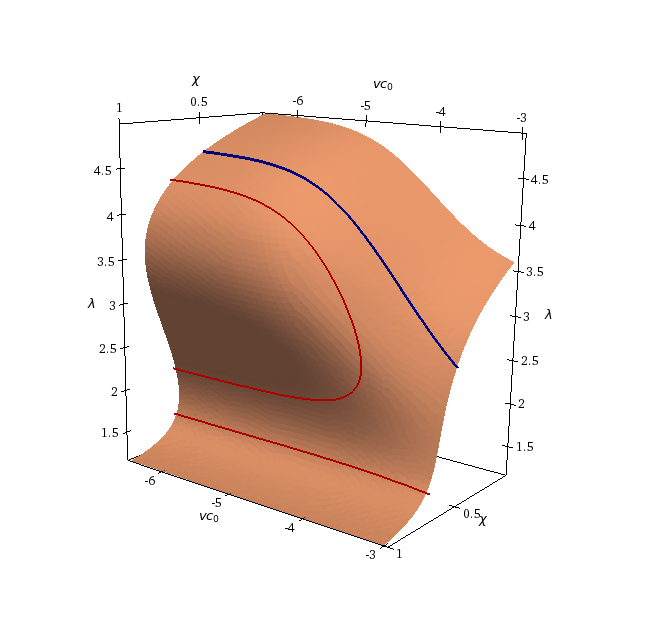
\includegraphics[scale=0.5]{images/manifold_new}
	\caption{Two-parameters bifurcation analysis: equilibrium manifold. The red line corresponds to the section of the manifold for $\chi=0.7$, while the blue line $\chi=0.5$.}
	\label{manifold}
\end{figure}
For the free swelling case the deformation tensor $\F=\lambda\mathbb{I}$ so that $\mathbb{B}=\lambda^2\mathbb{I}$. As in the paper by Yu, we now assume that $v=v_s$ so that the equations further simplify to:
\begin{gather}
\begin{aligned}
0 = p v + k_BT\left[\ln (c_s v) +2c_0v+
\frac{\chi(1-c_sv)+1}{J}\right], 
\end{aligned}\\[2.5mm]
z_f\frac{C_f}{J}+c_+-c_-=0,\\
0 = p v \pm e\Phi + k_BT \left(\ln \frac{c_\pm}{c_0}+2vc_0+\frac{1-\chi c_sv}{J} \right),\label{temp4}\\
p= \frac{G}{\lambda^3}\left(\lambda^2-1\right).
\end{gather}
Using Equations(68), we have that the electric potential has the form:
\begin{equation}
\Phi= \frac{k_BT}{2e}\ln\frac{C_-}{C_+}.
\end{equation}
while the concentrations $C_+$ and $C_-$, using also Equation~(\ref{temp4}):
\begin{gather}
C_- = c_0 C_s v \exp\left(\frac{e\Phi}{k_BT}+\frac{\chi}{J}\right),\\
C_+ = c_0 C_s v \exp\left(-\frac{e\Phi}{k_BT}+\frac{\chi}{J}\right).
\end{gather}
which implies that:
\begin{equation}
C_+C_-= c^2_0C^2_sv^2 \exp\left(\frac{2\chi}{J}\right).\label{mult}
\end{equation}
Combining~(\ref{mult}) with the electro-neutrality condition, we have:
\begin{equation}
C_\pm = \mp \frac{z_fC_f}{2} + \sqrt{\left( \frac{z_fC_f}{2} \right)^2 + c^2_0C_s^2 v^2 \exp\left(2\frac{\chi}{J}\right)}.
\end{equation}
Using the incompressibility condition, we have that:
\begin{equation}
\lambda^3=J=1+vC_s+vC_++vC_-.
\end{equation}
Finally substituting the definition of $p$ into Equation~(\ref{temp1}),we have:
\begin{eqnarray}
0=\frac{Gv}{k_BT\lambda^3}(\lambda^2-1) + 2c_0v + \ln (c_s v) +2c_0v+
\frac{\chi(1-c_sv)+1}{\lambda^3}\label{cond1}\\
\frac{\lambda^3-1}{\lambda^3}=vc_s+2\sqrt{\left( \frac{z_fC_f}{2\lambda^3} \right)^2 + c^2_0c_s^2 v^2 \exp\left(2\frac{\chi}{\lambda^3}\right)}\label{cond2}
\end{eqnarray}

Note that the two conditions~(\ref{cond1}) and (\ref{cond2}) uniquely define the equilibrium swelling ration for any value of $c_0$. Fixing the values of the other parameter to match with the work of Yu and varying $vc_0$ and $\chi$, we obtained the manifold showed in Figure \ref{manifold}.

When considering the 1D case, the folding of the manifold is less prominent. However there are sets of parameters for which a similar collapse can be observed, as shown in Figure \ref{manifold2}.
\begin{figure}[h]
	\begin{subfigure}{0.49\textwidth}
		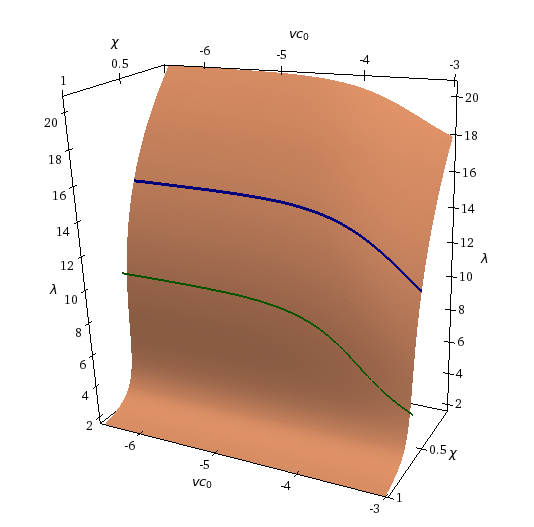
\includegraphics[scale=0.4]{images/manifold1D_2}
		\caption{$C_f=0.02$}
	\end{subfigure}
\hspace{5mm}
	\begin{subfigure}{0.49\textwidth}
		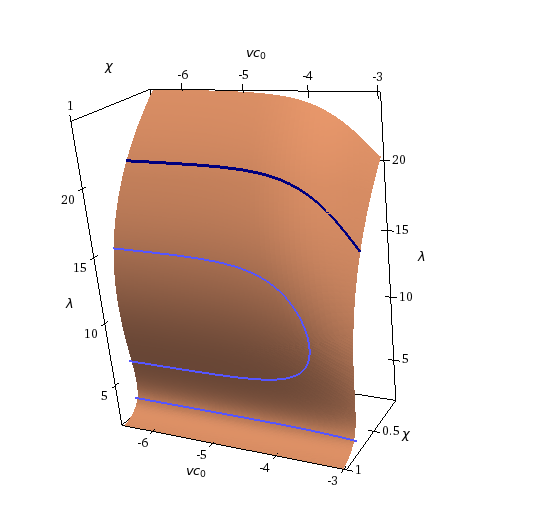
\includegraphics[scale=0.45]{images/manifold1D_1}
		\caption{$C_f=0.04$}
	\end{subfigure}
	\caption{Two-parameters bifurcation analysis: equilibrium manifold. The purple line corresponds to the section of the manifold for $\chi=0.8$, the green line $\chi=0.65$, while the blue line $\chi=0.5$.}
	\label{manifold2}
\end{figure}
